\documentclass[]{book}
\usepackage{lmodern}
\usepackage{amssymb,amsmath}
\usepackage{ifxetex,ifluatex}
\usepackage{fixltx2e} % provides \textsubscript
\ifnum 0\ifxetex 1\fi\ifluatex 1\fi=0 % if pdftex
  \usepackage[T1]{fontenc}
  \usepackage[utf8]{inputenc}
\else % if luatex or xelatex
  \ifxetex
    \usepackage{mathspec}
  \else
    \usepackage{fontspec}
  \fi
  \defaultfontfeatures{Ligatures=TeX,Scale=MatchLowercase}
\fi
% use upquote if available, for straight quotes in verbatim environments
\IfFileExists{upquote.sty}{\usepackage{upquote}}{}
% use microtype if available
\IfFileExists{microtype.sty}{%
\usepackage{microtype}
\UseMicrotypeSet[protrusion]{basicmath} % disable protrusion for tt fonts
}{}
\usepackage[margin=1in]{geometry}
\usepackage{hyperref}
\hypersetup{unicode=true,
            pdftitle={Data Mining for Student Success and Perseverance},
            pdfauthor={Sameer Bhatnagar; Jonathan Guillemette; Micheal Dugdale; Sahir Bhatnagar; Nathaniel Lasry},
            pdfborder={0 0 0},
            breaklinks=true}
\urlstyle{same}  % don't use monospace font for urls
\usepackage{natbib}
\bibliographystyle{apalike}
\usepackage{longtable,booktabs}
\usepackage{graphicx,grffile}
\makeatletter
\def\maxwidth{\ifdim\Gin@nat@width>\linewidth\linewidth\else\Gin@nat@width\fi}
\def\maxheight{\ifdim\Gin@nat@height>\textheight\textheight\else\Gin@nat@height\fi}
\makeatother
% Scale images if necessary, so that they will not overflow the page
% margins by default, and it is still possible to overwrite the defaults
% using explicit options in \includegraphics[width, height, ...]{}
\setkeys{Gin}{width=\maxwidth,height=\maxheight,keepaspectratio}
\IfFileExists{parskip.sty}{%
\usepackage{parskip}
}{% else
\setlength{\parindent}{0pt}
\setlength{\parskip}{6pt plus 2pt minus 1pt}
}
\setlength{\emergencystretch}{3em}  % prevent overfull lines
\providecommand{\tightlist}{%
  \setlength{\itemsep}{0pt}\setlength{\parskip}{0pt}}
\setcounter{secnumdepth}{5}
% Redefines (sub)paragraphs to behave more like sections
\ifx\paragraph\undefined\else
\let\oldparagraph\paragraph
\renewcommand{\paragraph}[1]{\oldparagraph{#1}\mbox{}}
\fi
\ifx\subparagraph\undefined\else
\let\oldsubparagraph\subparagraph
\renewcommand{\subparagraph}[1]{\oldsubparagraph{#1}\mbox{}}
\fi

%%% Use protect on footnotes to avoid problems with footnotes in titles
\let\rmarkdownfootnote\footnote%
\def\footnote{\protect\rmarkdownfootnote}

%%% Change title format to be more compact
\usepackage{titling}

% Create subtitle command for use in maketitle
\newcommand{\subtitle}[1]{
  \posttitle{
    \begin{center}\large#1\end{center}
    }
}

\setlength{\droptitle}{-2em}
  \title{Data Mining for Student Success and Perseverance}
  \pretitle{\vspace{\droptitle}\centering\huge}
  \posttitle{\par}
  \author{Sameer Bhatnagar \\ Jonathan Guillemette \\ Micheal Dugdale \\ Sahir Bhatnagar \\ Nathaniel Lasry}
  \preauthor{\centering\large\emph}
  \postauthor{\par}
  \predate{\centering\large\emph}
  \postdate{\par}
  \date{2017-10-27}

\usepackage{booktabs}
\usepackage{amsthm}
\makeatletter
\def\thm@space@setup{%
  \thm@preskip=8pt plus 2pt minus 4pt
  \thm@postskip=\thm@preskip
}
\makeatother

\usepackage{amsthm}
\newtheorem{theorem}{Theorem}[chapter]
\newtheorem{lemma}{Lemma}[chapter]
\theoremstyle{definition}
\newtheorem{definition}{Definition}[chapter]
\newtheorem{corollary}{Corollary}[chapter]
\newtheorem{proposition}{Proposition}[chapter]
\theoremstyle{definition}
\newtheorem{example}{Example}[chapter]
\theoremstyle{remark}
\newtheorem*{remark}{Remark}
\begin{document}
\maketitle

{
\setcounter{tocdepth}{1}
\tableofcontents
}
\chapter{Preface}\label{preface}

This report summarizes the work done by our team on using college
registration records at three diffrenet anglophone CEGEPS in Montreal in
order to find predictors of attrition.

\chapter{Introduction}\label{intro}

\section{Context}\label{context}

This report outlines the results from a three year intercollegiate
research project funded by the\textbf{PAREA} agency ( \emph{Programmme
d'Aide à la Recherche en Enseignment et Apprentissage}) from the
\emph{Ministère de l'Education} of the provincial Government of Quebec.

In the province of Quebec, students finish their secondary education at
what is the equivalent of Grade 11 in other parts of North America.
Students are then able to attend \textbf{CEGEP} ( \emph{Collège
d'enseignment général et professionel}) for either

\begin{itemize}
\tightlist
\item
  two years, as part of pre-university program, e.g Science, Social
  Science, Liberal Arts
\item
  three years, as part of technical program, meant specifically to lead
  directly to the job market, e.g.~Nursing, Civil Engineering
  Technology, Diagnotsic Imaging Technology
\end{itemize}

There are 48 CEGEPs in the Quebec network, and public or private, they
all fall under the purview of the \emph{Ministère de l'Education et
Enseignment Superieur}. Over the past twenty years, there has been
significant
work\citep{jorgensen2003students, jorgensen2005academic, jorgensen2009predicting, riviere1995decrocheurs, shaienks2008statcan}
and media
\citep{breton2016soleil, dion-viens2015lapresse, duchaine2017lapresse}
on the topic of student attrition in CEGEP. The scholarly work done has
often focused on determing predictors of attrition through surveys, or
focused on specific vulnerable sub populations. The media has often
reported on government figures, which rely on data that looks at
information at a very coarse level of granularity (of students graduated
from high schoolhow many obtain diplomas from CEGEP)

\section{Objectives}\label{objectives}

Almost all of the CEGEP's use the same database system, known as
\textbf{CLARA} (developped by the company Skytech) in order to manage
the data related to student admission, registration and graduation. Our
research team's main objective is to leverage this uniformity of how
data is automatically generated and stored, in order to determine if, in
this wealth of data, there might be predictors of student attrition.
This effort stands apart from previous work and reports in that:

\begin{itemize}
\tightlist
\item
  the data analyzed is much finer-grained: the unit of analysis is down
  to the semester registration records for each student
\item
  we look at the general population of students
\item
  to our knowledge, this is the first ever such study to span multiple
  CEGEPs, which we hope adds a greater relibility and validity to our
  findings.
\end{itemize}

This project has two specific objectives:

\begin{enumerate}
\def\labelenumi{\arabic{enumi})}
\tightlist
\item
  find predictors of students dropping out, whether they be demographic,
  or based in academic performance, on a term by term basis.
\item
  evaluate methods by which students can be automatically flagged as
  being at risk of dropping out, without so much a focus on
  understanding why, but for the purpose of ``general offers of
  support'' or further investigation
\end{enumerate}

This report is structured to reflect these two objectives. Namely, we
begin with - a standard review of previous
\protect\hyperlink{littreview}{related work}, - a section on
\protect\hyperlink{descriptive}{descriptive statistics} which gives an
overview of the dataset.

We then move on to our methods and models over two chapters: - the
\protect\hyperlink{explanatory}{first} addresses objective 1, outlining
our efforts to find explanatory predictors of student attrition in
classical statistical models. - The
\protect\hyperlink{predictive}{following chapter} addresses objective 2,
describing modern methods from the field of machine learning, which, at
the expense of model interpretability, are fit to provide maximum
predictive accuracy in identifying students at-risk.

The report then concludes with -
\protect\hyperlink{comparisons}{comparisons} of these methods with each
other, and to current intervention frameworks in place at participating
colleges - an auxilliary chapter looking at students from the division
of \protect\hyperlink{conted}{Continuing Education} - a
\protect\hyperlink{conclusion}{concluding chapter}, with reccomendations
for future directions

\hypertarget{littreview}{\chapter{Literature}\label{littreview}}

\textbf{Under Construction }

\section{Modeling success and attrition in
CEGEP}\label{modeling-success-and-attrition-in-cegep}

The most important relevant work for this project is
{[}\citep{jorgensen2009pareafinalreport}{]}.

\section{Predictive Modelling in Learning Analytics and Educational Data
Mining}\label{predictive-modelling-in-learning-analytics-and-educational-data-mining}

\citep{hla2017}

\hypertarget{descriptive}{\chapter{Descriptive
Statistics}\label{descriptive}}

** Under Construction **

Here in we will describe - the data set - the methods by which we label
students at risk - the distributions of at-risk students by -
demographic indicators - registration record indicators

\section{Demographics across the colleges and major
programs}\label{demographics-across-the-colleges-and-major-programs}

\subsection{Dawson}\label{dawson}

\begin{longtable}[]{@{}ccccc@{}}
\toprule
\begin{minipage}[b]{0.12\columnwidth}\centering\strut
~\strut
\end{minipage} & \begin{minipage}[b]{0.06\columnwidth}\centering\strut
AN\strut
\end{minipage} & \begin{minipage}[b]{0.06\columnwidth}\centering\strut
AU\strut
\end{minipage} & \begin{minipage}[b]{0.06\columnwidth}\centering\strut
FR\strut
\end{minipage} & \begin{minipage}[b]{0.06\columnwidth}\centering\strut
Sum\strut
\end{minipage}\tabularnewline
\midrule
\endhead
\begin{minipage}[t]{0.12\columnwidth}\centering\strut
\textbf{F}\strut
\end{minipage} & \begin{minipage}[t]{0.06\columnwidth}\centering\strut
0.33\strut
\end{minipage} & \begin{minipage}[t]{0.06\columnwidth}\centering\strut
0.15\strut
\end{minipage} & \begin{minipage}[t]{0.06\columnwidth}\centering\strut
0.12\strut
\end{minipage} & \begin{minipage}[t]{0.06\columnwidth}\centering\strut
0.6\strut
\end{minipage}\tabularnewline
\begin{minipage}[t]{0.12\columnwidth}\centering\strut
\textbf{M}\strut
\end{minipage} & \begin{minipage}[t]{0.06\columnwidth}\centering\strut
0.23\strut
\end{minipage} & \begin{minipage}[t]{0.06\columnwidth}\centering\strut
0.1\strut
\end{minipage} & \begin{minipage}[t]{0.06\columnwidth}\centering\strut
0.07\strut
\end{minipage} & \begin{minipage}[t]{0.06\columnwidth}\centering\strut
0.4\strut
\end{minipage}\tabularnewline
\begin{minipage}[t]{0.12\columnwidth}\centering\strut
\textbf{Sum}\strut
\end{minipage} & \begin{minipage}[t]{0.06\columnwidth}\centering\strut
0.56\strut
\end{minipage} & \begin{minipage}[t]{0.06\columnwidth}\centering\strut
0.25\strut
\end{minipage} & \begin{minipage}[t]{0.06\columnwidth}\centering\strut
0.19\strut
\end{minipage} & \begin{minipage}[t]{0.06\columnwidth}\centering\strut
1\strut
\end{minipage}\tabularnewline
\bottomrule
\end{longtable}

\subsection{John Abbott College}\label{john-abbott-college}

\begin{longtable}[]{@{}ccccc@{}}
\toprule
\begin{minipage}[b]{0.12\columnwidth}\centering\strut
~\strut
\end{minipage} & \begin{minipage}[b]{0.06\columnwidth}\centering\strut
AN\strut
\end{minipage} & \begin{minipage}[b]{0.06\columnwidth}\centering\strut
AU\strut
\end{minipage} & \begin{minipage}[b]{0.06\columnwidth}\centering\strut
FR\strut
\end{minipage} & \begin{minipage}[b]{0.06\columnwidth}\centering\strut
Sum\strut
\end{minipage}\tabularnewline
\midrule
\endhead
\begin{minipage}[t]{0.12\columnwidth}\centering\strut
\textbf{F}\strut
\end{minipage} & \begin{minipage}[t]{0.06\columnwidth}\centering\strut
0.31\strut
\end{minipage} & \begin{minipage}[t]{0.06\columnwidth}\centering\strut
0.09\strut
\end{minipage} & \begin{minipage}[t]{0.06\columnwidth}\centering\strut
0.12\strut
\end{minipage} & \begin{minipage}[t]{0.06\columnwidth}\centering\strut
0.52\strut
\end{minipage}\tabularnewline
\begin{minipage}[t]{0.12\columnwidth}\centering\strut
\textbf{M}\strut
\end{minipage} & \begin{minipage}[t]{0.06\columnwidth}\centering\strut
0.3\strut
\end{minipage} & \begin{minipage}[t]{0.06\columnwidth}\centering\strut
0.07\strut
\end{minipage} & \begin{minipage}[t]{0.06\columnwidth}\centering\strut
0.11\strut
\end{minipage} & \begin{minipage}[t]{0.06\columnwidth}\centering\strut
0.48\strut
\end{minipage}\tabularnewline
\begin{minipage}[t]{0.12\columnwidth}\centering\strut
\textbf{Sum}\strut
\end{minipage} & \begin{minipage}[t]{0.06\columnwidth}\centering\strut
0.61\strut
\end{minipage} & \begin{minipage}[t]{0.06\columnwidth}\centering\strut
0.16\strut
\end{minipage} & \begin{minipage}[t]{0.06\columnwidth}\centering\strut
0.23\strut
\end{minipage} & \begin{minipage}[t]{0.06\columnwidth}\centering\strut
1\strut
\end{minipage}\tabularnewline
\bottomrule
\end{longtable}

\subsection{Vanier}\label{vanier}

\begin{longtable}[]{@{}ccccc@{}}
\toprule
\begin{minipage}[b]{0.12\columnwidth}\centering\strut
~\strut
\end{minipage} & \begin{minipage}[b]{0.06\columnwidth}\centering\strut
AN\strut
\end{minipage} & \begin{minipage}[b]{0.06\columnwidth}\centering\strut
AU\strut
\end{minipage} & \begin{minipage}[b]{0.06\columnwidth}\centering\strut
FR\strut
\end{minipage} & \begin{minipage}[b]{0.06\columnwidth}\centering\strut
Sum\strut
\end{minipage}\tabularnewline
\midrule
\endhead
\begin{minipage}[t]{0.12\columnwidth}\centering\strut
\textbf{F}\strut
\end{minipage} & \begin{minipage}[t]{0.06\columnwidth}\centering\strut
0.26\strut
\end{minipage} & \begin{minipage}[t]{0.06\columnwidth}\centering\strut
0.17\strut
\end{minipage} & \begin{minipage}[t]{0.06\columnwidth}\centering\strut
0.1\strut
\end{minipage} & \begin{minipage}[t]{0.06\columnwidth}\centering\strut
0.53\strut
\end{minipage}\tabularnewline
\begin{minipage}[t]{0.12\columnwidth}\centering\strut
\textbf{M}\strut
\end{minipage} & \begin{minipage}[t]{0.06\columnwidth}\centering\strut
0.24\strut
\end{minipage} & \begin{minipage}[t]{0.06\columnwidth}\centering\strut
0.16\strut
\end{minipage} & \begin{minipage}[t]{0.06\columnwidth}\centering\strut
0.08\strut
\end{minipage} & \begin{minipage}[t]{0.06\columnwidth}\centering\strut
0.48\strut
\end{minipage}\tabularnewline
\begin{minipage}[t]{0.12\columnwidth}\centering\strut
\textbf{Sum}\strut
\end{minipage} & \begin{minipage}[t]{0.06\columnwidth}\centering\strut
0.5\strut
\end{minipage} & \begin{minipage}[t]{0.06\columnwidth}\centering\strut
0.33\strut
\end{minipage} & \begin{minipage}[t]{0.06\columnwidth}\centering\strut
0.18\strut
\end{minipage} & \begin{minipage}[t]{0.06\columnwidth}\centering\strut
1.01\strut
\end{minipage}\tabularnewline
\bottomrule
\end{longtable}

\section{Academic Performance in Semesters leading to
drop-out}\label{academic-performance-in-semesters-leading-to-drop-out}

\subsection{Grades}\label{grades}

Do students who drop out do so because of poor grades? What fraction of
students are counted year after year as drop-outs and labeled as
problems to be solved by the system while being exemplary students in
terms of academic performance. Armed with this dataset, we can get the
answer to that question. Let us begin by looking at the average grades
of students who eventually dropped out compared to grades of students
who haven't. The following set of graphs will look at that comparison
for 3 different semesters: the semester in which they dropped out (or
graduated), the semester before that and the one before that. Let us see
what the data says.

\includegraphics{studentsuccess_final_report_files/figure-latex/Average comp-1.pdf}

From the average total grade between the drop outs and the graduates, we
can clearly see that the distributions are significantly different, but
what is surprising is that NaN\% of students have an average grade above
75\% and that more than NaN\% of the students who dropped out had an
average grade above 60\%. In other words, most students who drop out
have passing averages. One hypothesis for this effect is that students
who end up dropping out start with good semesters and have their
performance decline closer to the final semester. Let us verify this
hypothesis.

Let us now look at the performance of drop outs vs graduates on a
semester by semester basis. Let us start by looking at the average
grades of students in their last semester during which they are either
graduating or dropping-out.
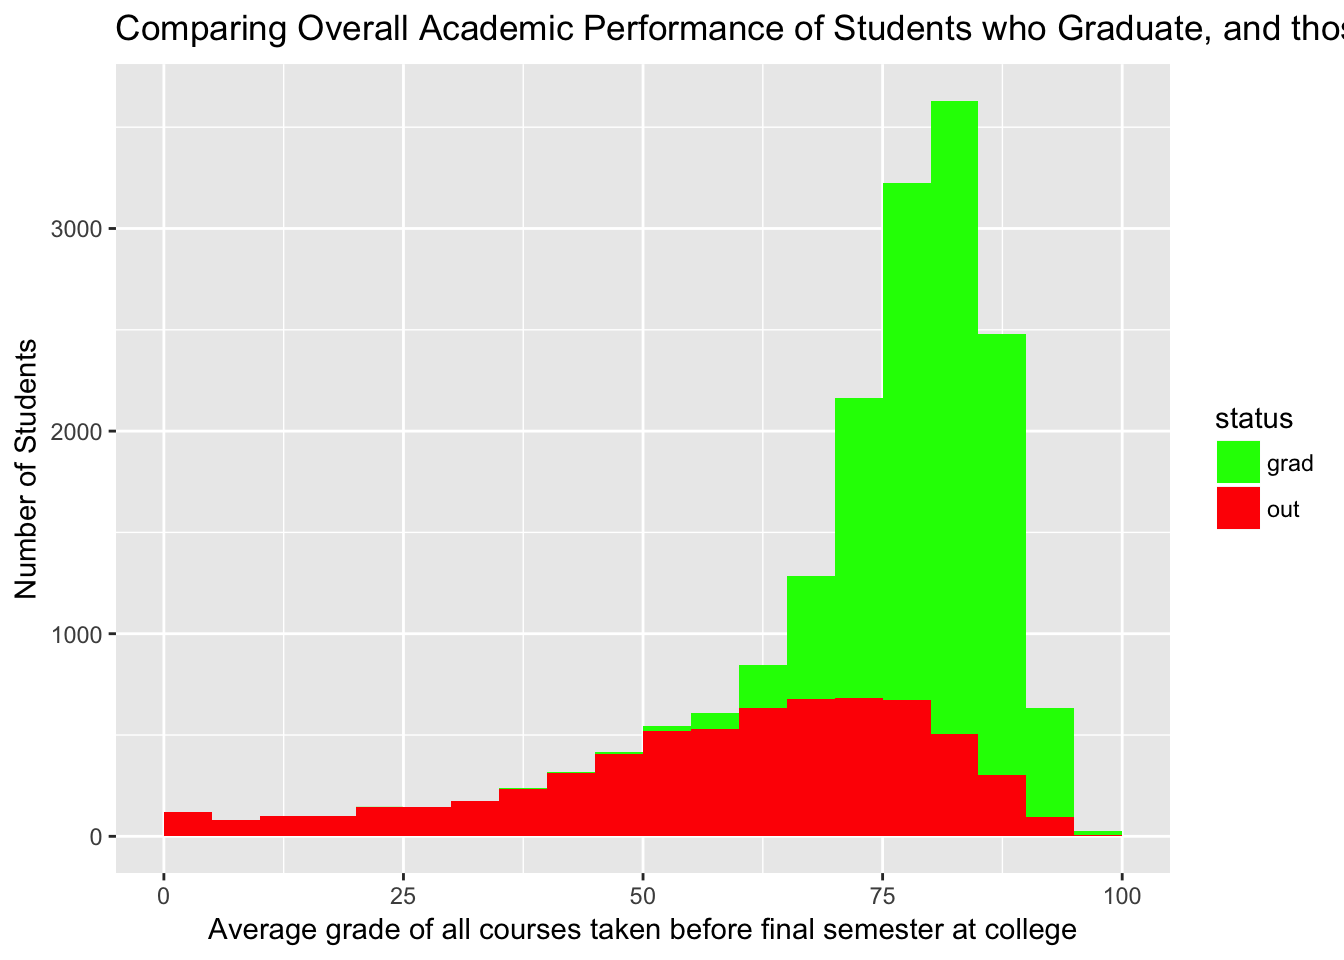
\includegraphics{studentsuccess_final_report_files/figure-latex/Average-comp-1.pdf}

\begin{verbatim}
## 
##  Welch Two Sample t-test
## 
## data:  Average_all_courses by status
## t = 78.251, df = 7349.6, p-value < 2.2e-16
## alternative hypothesis: true difference in means is not equal to 0
## 95 percent confidence interval:
##  20.36923 21.41600
## sample estimates:
## mean in group grad  mean in group out 
##           79.97370           59.08109
\end{verbatim}

From the average total grade between the drop outs and the graduates, we
can clearly see that the distributions are significantly different, but
what is surprising is that 22\% of students have an average grade above
75\% and that more than 52\% of the students who dropped out had an
average grade above 60\%. In other words, most students who drop out
have passing averages. One hypothesis for this effect is that students
who end up dropping out start with good semesters and have their
performance decline closer to the final semester. Let us verify this
hypothesis.

Let us now look at the performance of drop outs vs graduates on a
semester by semester basis. Let us start by looking at the average
grades of students in their last semester during which they are either
graduating or dropping-out.

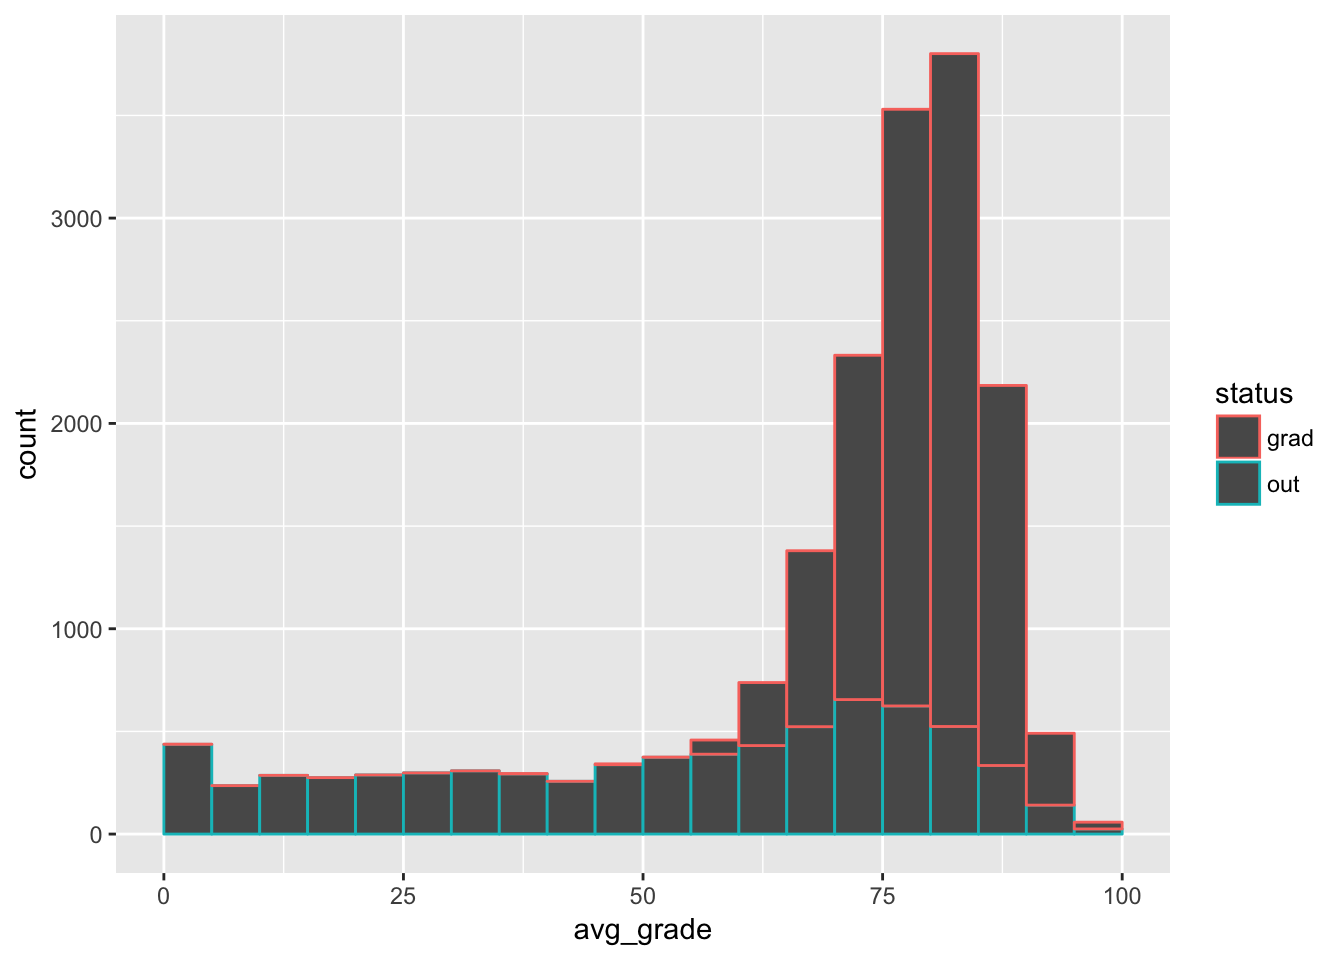
\includegraphics{studentsuccess_final_report_files/figure-latex/Last-semester-comp-1.pdf}

\begin{verbatim}
## 
##  Welch Two Sample t-test
## 
## data:  avg_grade by status
## t = 84.649, df = 7619.5, p-value < 2.2e-16
## alternative hypothesis: true difference in means is not equal to 0
## 95 percent confidence interval:
##  27.00250 28.28279
## sample estimates:
## mean in group grad  mean in group out 
##           79.17656           51.53391
\end{verbatim}

In this data, we can clearly observe a stark difference between the
graduates and the drop outs. First of all, note that 23\% of students
still have a term average over 75\% in the semester in which they drop
out. To push it further 15\% of students who drop out have an average
grade over 80\%. The data clearly suggests that some of the drop outs
aren't dropping out because of academic performance. Furthermore, the
long tail of the data on the low end of performance suggests that some
of the students stopped coming to class prior to the end of the semester
resulting in very low grades that serve to drive their cegep average
grades from the graph above even lower. 34\% of students have a grade
below 40 suggesting that they have indeed stopped coming to school some
time during the semester. What if these students hadn't stopped coming,
would their performance be similar to that of graduates?

Let us now turn our attention to the semester before the one where they
graduate or drop out.

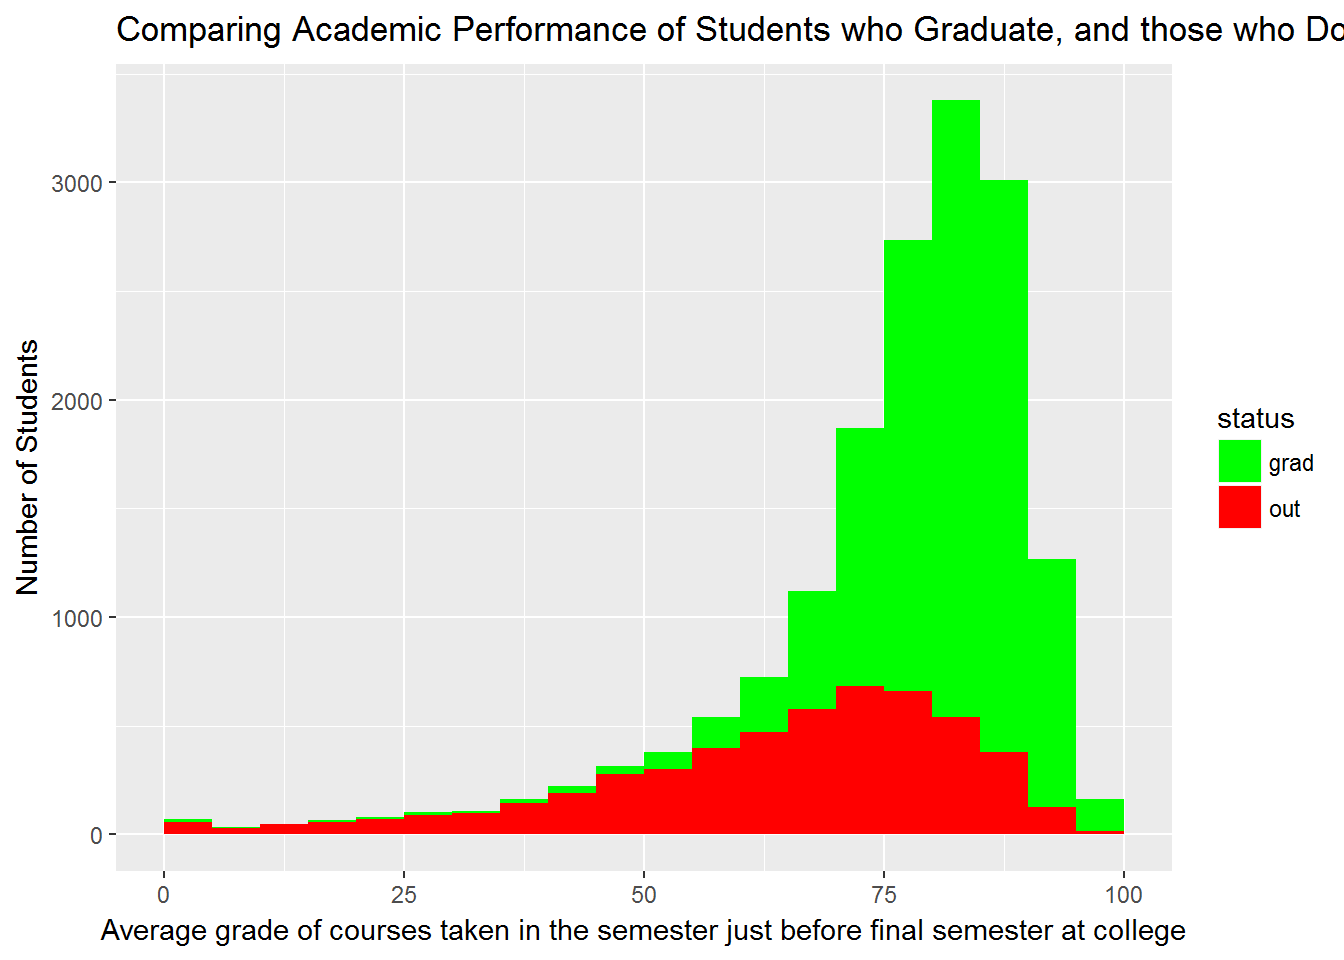
\includegraphics{studentsuccess_final_report_files/figure-latex/N-1-semester-comp-1.pdf}

In this data, we can clearly observe a stark difference between the
graduates and the drop outs. First of all, note that 22\% of students
still have a term average over 75\% in the semester in which they drop
out. To push it further 14\% of students who drop out have an average
grade over 80\%. The data clearly suggests that some of the drop outs
aren't dropping out because of academic performance. Furthermore, the
long tail of the data on the low end of performance suggests that some
of the students stopped coming to class prior to the end of the semester
resulting in very low grades that serve to drive their cegep average
grades from the graph above even lower. 34\% of students have a grade
below 40 suggesting that they have indeed stopped coming to school some
time during the semester. What if these students hadn't stopped coming,
would their performance be similar to that of graduates?

Let us now turn our attention to the semester before the one where they
graduate or drop out.

\begin{verbatim}
## 
##  Welch Two Sample t-test
## 
## data:  avg_grade by status
## t = 57.702, df = 6604.9, p-value < 2.2e-16
## alternative hypothesis: true difference in means is not equal to 0
## 95 percent confidence interval:
##  15.65690 16.75814
## sample estimates:
## mean in group grad  mean in group out 
##           80.56981           64.36230
\end{verbatim}

The data clearly shows that even if there are significant differences
between the groups, the drop out student population is getting closer to
the graduate population. A section of 33\% is observed to have an
average grade above 75\%.

Finally, let us look at 2 semesters before they graduate or drop-out. We
are again expecting the same trend.

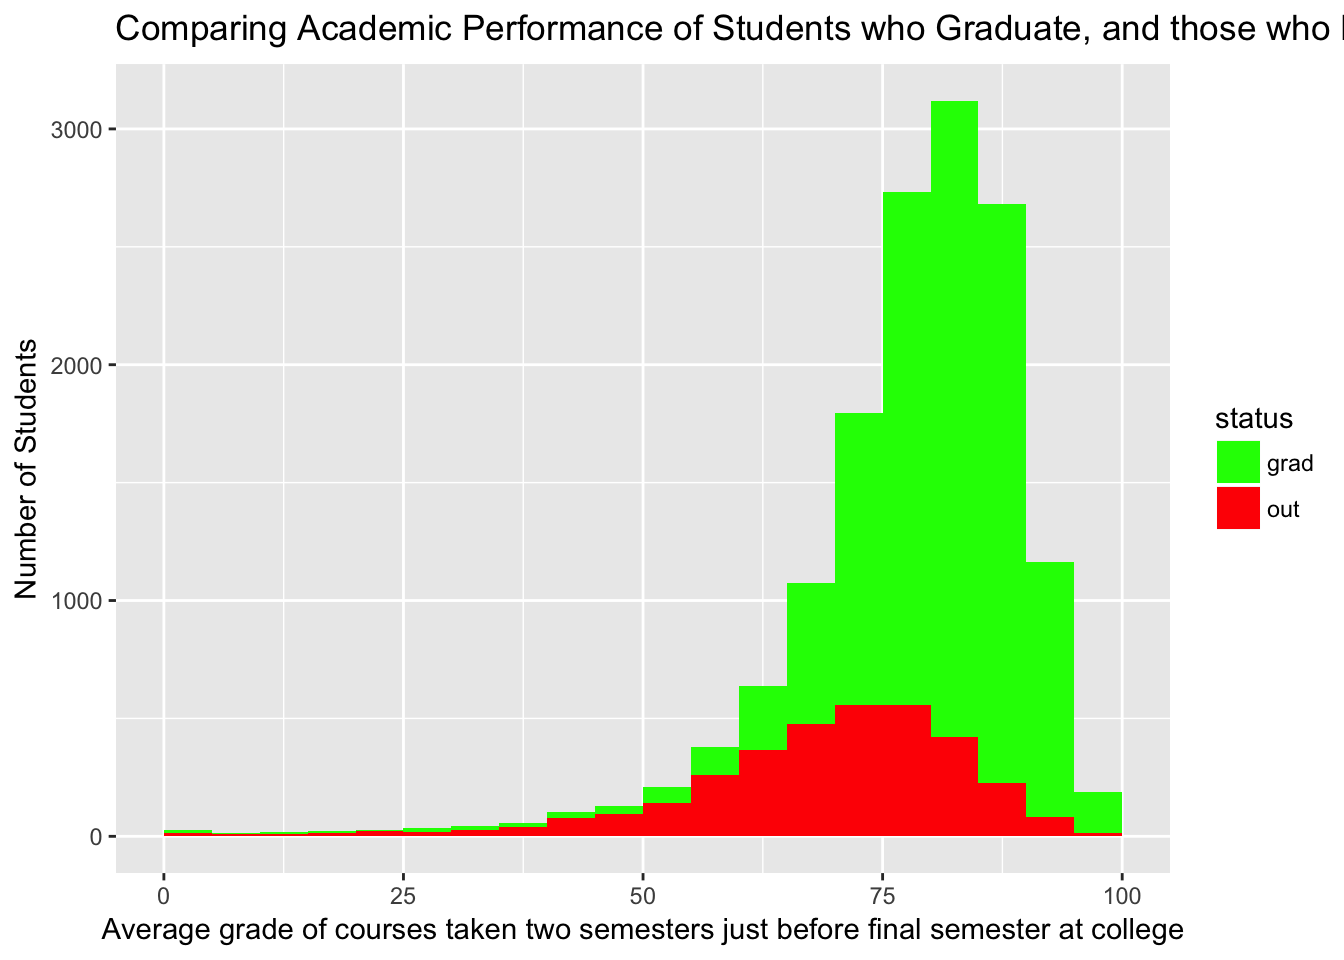
\includegraphics{studentsuccess_final_report_files/figure-latex/N-2-semester-comp-1.pdf}

\begin{verbatim}
## 
##  Welch Two Sample t-test
## 
## data:  avg_grade by status
## t = 42.166, df = 4390.4, p-value < 2.2e-16
## alternative hypothesis: true difference in means is not equal to 0
## 95 percent confidence interval:
##  10.95430 12.02262
## sample estimates:
## mean in group grad  mean in group out 
##           80.42574           68.93729
\end{verbatim}

\hypertarget{conclusion}{\section{Conclusion}\label{conclusion}}

In conclusion, the data strongly suggests that there are approximately
20\% of students who consistently have averages above 75\%, but still
drop out. Therefore, that section of the drop out population is a
section that will always go undetected if only traditional academic
failure metrics are used to assess which students are likely to drop
out. Students who move out to the US or the rest of Canada after their
second semester and those who drop out by lack of interest are two
potential student types that will always drop out no matter what
remedial solutions are offered for them.

One of the profile level Key Performance Indicators that colleges are
supposed to specifically keep track of is third semester retention. In
this light, we can somewhat flip the line of questionning above, and
look to see if the distribution of grades in the third semester students
looks different for those who will drop out, and those who will continue
on.

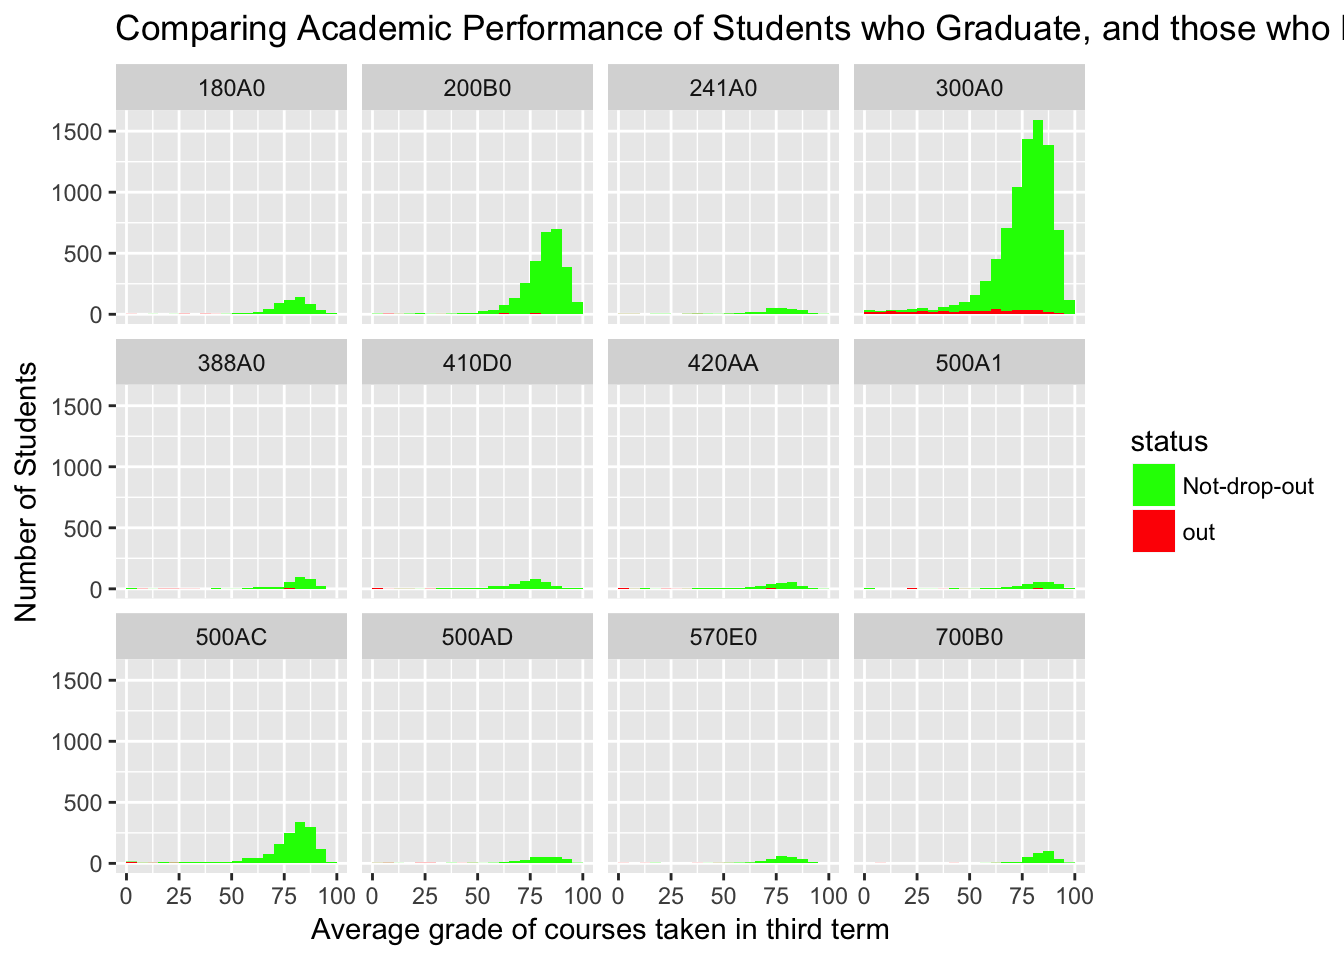
\includegraphics{studentsuccess_final_report_files/figure-latex/third-semester-attrition-by-program-1.pdf}

In conclusion, the data strongly suggests that there are approximately
20\% of students who consistently have averages above 75\%, but still
drop out. Therefore, that section of the drop out population is a
section that will always go undetected if only traditional academic
failure metrics are used to assess which students are likely to drop
out. Students who move out to the US or the rest of Canada after their
second semester and those who drop out by lack of interest are two
potential student types that will always drop out no matter what
remedial solutions are offered for them.

\subsection{Passed vs.~Failed Courses}\label{passed-vs.failed-courses}

The line of questionning above can be repeated, but instead of looking
at the average grade of courses taken in a term, we can instead look to
see if the number of courses passed, or the proportion failed, might be
different for students who drop out versus those who do not.

\begin{longtable}[]{@{}ccccccccccc@{}}
\toprule
\begin{minipage}[b]{0.19\columnwidth}\centering\strut
~\strut
\end{minipage} & \begin{minipage}[b]{0.06\columnwidth}\centering\strut
0\strut
\end{minipage} & \begin{minipage}[b]{0.05\columnwidth}\centering\strut
1\strut
\end{minipage} & \begin{minipage}[b]{0.04\columnwidth}\centering\strut
2\strut
\end{minipage} & \begin{minipage}[b]{0.04\columnwidth}\centering\strut
3\strut
\end{minipage} & \begin{minipage}[b]{0.04\columnwidth}\centering\strut
4\strut
\end{minipage} & \begin{minipage}[b]{0.04\columnwidth}\centering\strut
5\strut
\end{minipage} & \begin{minipage}[b]{0.04\columnwidth}\centering\strut
6\strut
\end{minipage} & \begin{minipage}[b]{0.04\columnwidth}\centering\strut
7\strut
\end{minipage} & \begin{minipage}[b]{0.04\columnwidth}\centering\strut
8\strut
\end{minipage} & \begin{minipage}[b]{0.04\columnwidth}\centering\strut
10\strut
\end{minipage}\tabularnewline
\midrule
\endhead
\begin{minipage}[t]{0.19\columnwidth}\centering\strut
\textbf{Not-drop-out}\strut
\end{minipage} & \begin{minipage}[t]{0.06\columnwidth}\centering\strut
11339\strut
\end{minipage} & \begin{minipage}[t]{0.05\columnwidth}\centering\strut
1320\strut
\end{minipage} & \begin{minipage}[t]{0.04\columnwidth}\centering\strut
447\strut
\end{minipage} & \begin{minipage}[t]{0.04\columnwidth}\centering\strut
216\strut
\end{minipage} & \begin{minipage}[t]{0.04\columnwidth}\centering\strut
116\strut
\end{minipage} & \begin{minipage}[t]{0.04\columnwidth}\centering\strut
66\strut
\end{minipage} & \begin{minipage}[t]{0.04\columnwidth}\centering\strut
34\strut
\end{minipage} & \begin{minipage}[t]{0.04\columnwidth}\centering\strut
8\strut
\end{minipage} & \begin{minipage}[t]{0.04\columnwidth}\centering\strut
2\strut
\end{minipage} & \begin{minipage}[t]{0.04\columnwidth}\centering\strut
0\strut
\end{minipage}\tabularnewline
\begin{minipage}[t]{0.19\columnwidth}\centering\strut
\textbf{out}\strut
\end{minipage} & \begin{minipage}[t]{0.06\columnwidth}\centering\strut
263\strut
\end{minipage} & \begin{minipage}[t]{0.05\columnwidth}\centering\strut
113\strut
\end{minipage} & \begin{minipage}[t]{0.04\columnwidth}\centering\strut
93\strut
\end{minipage} & \begin{minipage}[t]{0.04\columnwidth}\centering\strut
80\strut
\end{minipage} & \begin{minipage}[t]{0.04\columnwidth}\centering\strut
134\strut
\end{minipage} & \begin{minipage}[t]{0.04\columnwidth}\centering\strut
109\strut
\end{minipage} & \begin{minipage}[t]{0.04\columnwidth}\centering\strut
59\strut
\end{minipage} & \begin{minipage}[t]{0.04\columnwidth}\centering\strut
36\strut
\end{minipage} & \begin{minipage}[t]{0.04\columnwidth}\centering\strut
15\strut
\end{minipage} & \begin{minipage}[t]{0.04\columnwidth}\centering\strut
1\strut
\end{minipage}\tabularnewline
\bottomrule
\end{longtable}

What we remark in the table above is that the number of courses failed
does not seem to differentiate students who will drop out after their
third term. But perhaps, we should consider the fraction of courses that
a student took in their third term, and failed?

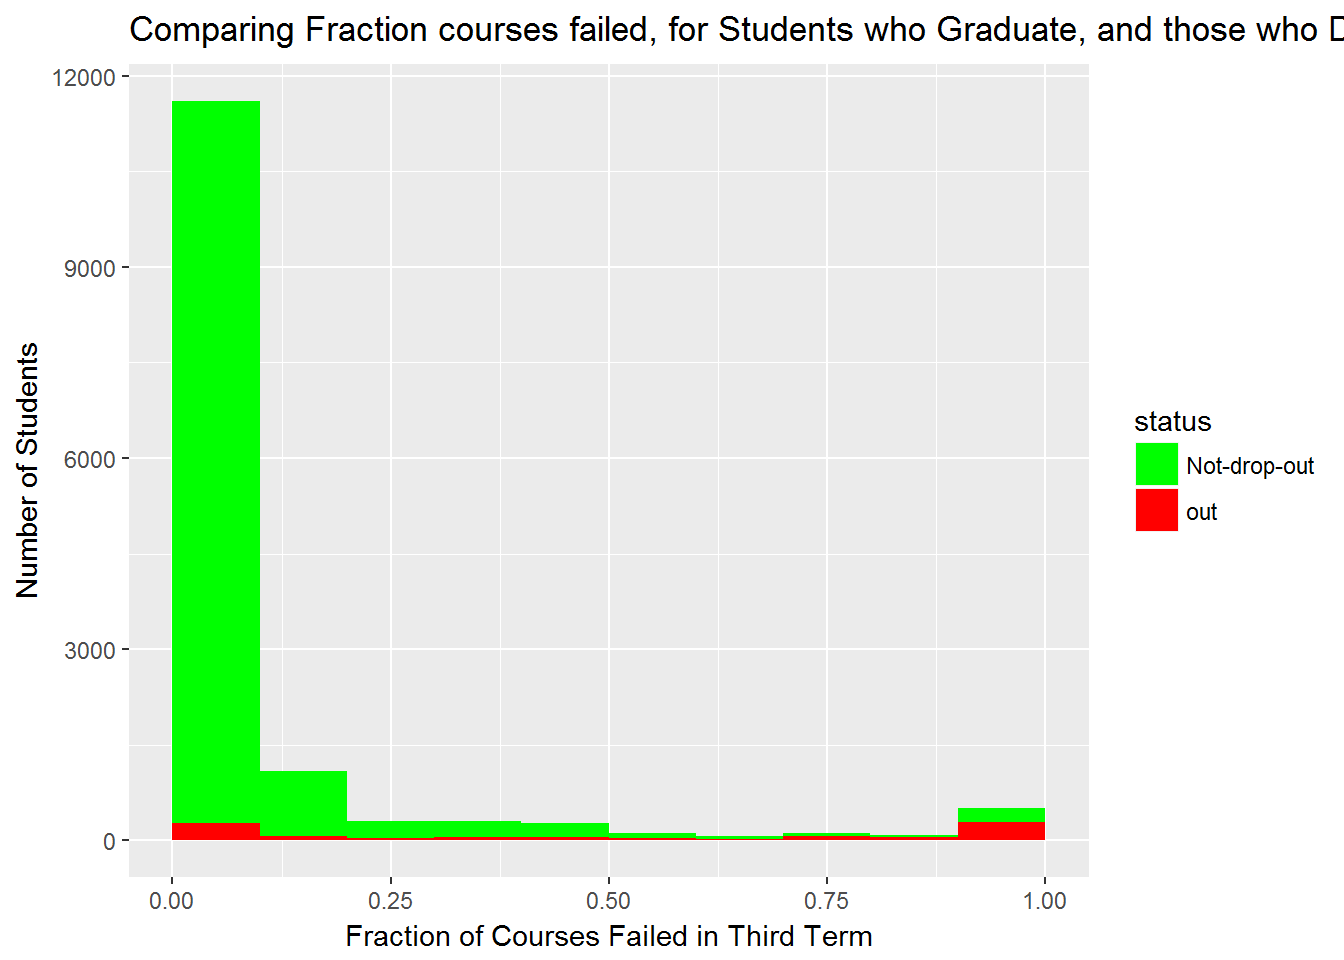
\includegraphics{studentsuccess_final_report_files/figure-latex/prop-failed-courses-1.pdf}

For the above graphic, we calculate, for each student in their term, the
fraction of courses that they took and \emph{failed}, and we plot the
distributions for the group of students we know who dropped out, and
those we know stayed in the college for a fourth term. The red boxplot
shows that,of the students who dropped out after their third term, 50\%
of them failed more than than half of their classes in that third term
(the central notch represents a 95\% confidence interval on the median).
Conversely, the distribution on the left, squashed down at 0, shows that
almost all students who stay on for a fourth term, pass all of their
third term classes (The additional dots shown in this distribution are
considered outliers to the distribution, meaning there are some students
who failed all of their third term classes, and decided to stay for an
additional fourth term).

\hypertarget{explanatory}{\chapter{Methods Centered on Determining
Predictive Factors}\label{explanatory}}

\textbf{Under Construction}

This chapter will be focused on methods which have a sound probabilistic
framework, and allow for inference into the statistical importance of
predictive factors.

\begin{itemize}
\tightlist
\item
  Logistic Regression
\item
  Mixed Effects Models
\end{itemize}

\hypertarget{predictive}{\chapter{Methods centered on predicting at-risk
students}\label{predictive}}

\textbf{Under construction}

Over the last twenty years, there has an increasing amount of work in
the applied social sciences that explore the use of what
\citep{breiman2001twocultures} refers to as ``algorithmic modelling''``,
as opposed to''data modelling``. He describes these as two cultures, the
former being made up of mostly computer scientists, and the latter being
made up statisticians (the methods therein are the ones explored in the
previous chapter of this report). The key metric in such classical
methods are \textbf{goodness of fit}, and such''explanatory``''
modelling aims to find associative and causal relationships between
predictors. Meanwhile, ``algorithmic''``, or''predictive``'' methods
emphasize determining any function that maps input variables to output
responses, with less regard for a probabilitic framework that allows for
causation, focusing solely on emprirical
precision\citep{shmueli2010explain}. In the recently published
\textbf{Handbok of Learning Analytics}\citep{hla2017}, published by the
Society of Learning Analytics Research, \citep{bergner_measurement_2017}
asserts that the researchers looking into educational data stand to gain
from understanding the nuances of both methodologies, as previous work
has shown the strengths and weakeness of either in this domain.

The previous chapter explored how classical statistical models can be
built and used to determine what are the factors that influence dropout.
This is useful for policy makers and admninstrators who want to dedicate
resources in the most strategic places. However this chapter will
explore models whose inner workings are less interpretable, but whose
primary objective is prediction/identification of at-risk students. This
is useful in the context where college administration has some blanket
intervention that it would like to apply, and we just want to ensure
that the students most in need are reached. Despite the less clear
interpratability of factors in these \emph{predictive} models (as
compared to the \emph{explanatory} models in the previous chapter), we
will stil explore methods to ``open up the black box'', and determine
which features are most important in achieving both accrate and
sensitive prediction.

\section{Decision Trees and Random
Forests}\label{decision-trees-and-random-forests}

\section{Neural Networks}\label{neural-networks}

\hypertarget{comparisons}{\chapter{Comparisons}\label{comparisons}}

** Under Construction **

This chapter will compare the effectiveness of the methods developped in
the previous two chapters, and compare them to more basic approaches to
identifying students at-risk.

For example, we know that some CEGEPs have implemented a policy whereby
they identify students as being at risk based on their mid-term
assessments: if the student receives a certain number of ``at-risk'' or
``failing'' results, they are automatically sent an email referring them
to academic support services.

Based on this, we can ask the following research questions : - how
effective is this approach at identifying students who drop-out? - how
does this approach compare to our models from the previous chapters?

We begin with a basic logistic regression with demographic variables,
and as well as the number of each type of results of mid-term
assessment, for students in their last term at the college. With these
predictors, we try to predict if students are about to graduate, or
simply not register again.

\begin{longtable}[]{@{}ccccc@{}}
\toprule
\begin{minipage}[b]{0.30\columnwidth}\centering\strut
~\strut
\end{minipage} & \begin{minipage}[b]{0.13\columnwidth}\centering\strut
Estimate\strut
\end{minipage} & \begin{minipage}[b]{0.16\columnwidth}\centering\strut
Std. Error\strut
\end{minipage} & \begin{minipage}[b]{0.12\columnwidth}\centering\strut
z value\strut
\end{minipage} & \begin{minipage}[b]{0.12\columnwidth}\centering\strut
Pr(\textgreater{}\textbar{}z\textbar{})\strut
\end{minipage}\tabularnewline
\midrule
\endhead
\begin{minipage}[t]{0.30\columnwidth}\centering\strut
\textbf{num\_pass}\strut
\end{minipage} & \begin{minipage}[t]{0.13\columnwidth}\centering\strut
0.5877\strut
\end{minipage} & \begin{minipage}[t]{0.16\columnwidth}\centering\strut
0.02321\strut
\end{minipage} & \begin{minipage}[t]{0.12\columnwidth}\centering\strut
25.32\strut
\end{minipage} & \begin{minipage}[t]{0.12\columnwidth}\centering\strut
1.747e-141\strut
\end{minipage}\tabularnewline
\begin{minipage}[t]{0.30\columnwidth}\centering\strut
\textbf{num\_at\_risk}\strut
\end{minipage} & \begin{minipage}[t]{0.13\columnwidth}\centering\strut
1.455\strut
\end{minipage} & \begin{minipage}[t]{0.16\columnwidth}\centering\strut
0.03664\strut
\end{minipage} & \begin{minipage}[t]{0.12\columnwidth}\centering\strut
39.7\strut
\end{minipage} & \begin{minipage}[t]{0.12\columnwidth}\centering\strut
0\strut
\end{minipage}\tabularnewline
\begin{minipage}[t]{0.30\columnwidth}\centering\strut
\textbf{num\_failing}\strut
\end{minipage} & \begin{minipage}[t]{0.13\columnwidth}\centering\strut
2.193\strut
\end{minipage} & \begin{minipage}[t]{0.16\columnwidth}\centering\strut
0.04653\strut
\end{minipage} & \begin{minipage}[t]{0.12\columnwidth}\centering\strut
47.15\strut
\end{minipage} & \begin{minipage}[t]{0.12\columnwidth}\centering\strut
0\strut
\end{minipage}\tabularnewline
\begin{minipage}[t]{0.30\columnwidth}\centering\strut
\textbf{num\_courses}\strut
\end{minipage} & \begin{minipage}[t]{0.13\columnwidth}\centering\strut
-0.7442\strut
\end{minipage} & \begin{minipage}[t]{0.16\columnwidth}\centering\strut
0.02373\strut
\end{minipage} & \begin{minipage}[t]{0.12\columnwidth}\centering\strut
-31.36\strut
\end{minipage} & \begin{minipage}[t]{0.12\columnwidth}\centering\strut
6.315e-216\strut
\end{minipage}\tabularnewline
\begin{minipage}[t]{0.30\columnwidth}\centering\strut
\textbf{SexeM}\strut
\end{minipage} & \begin{minipage}[t]{0.13\columnwidth}\centering\strut
0.2111\strut
\end{minipage} & \begin{minipage}[t]{0.16\columnwidth}\centering\strut
0.0386\strut
\end{minipage} & \begin{minipage}[t]{0.12\columnwidth}\centering\strut
5.469\strut
\end{minipage} & \begin{minipage}[t]{0.12\columnwidth}\centering\strut
4.537e-08\strut
\end{minipage}\tabularnewline
\begin{minipage}[t]{0.30\columnwidth}\centering\strut
\textbf{birth\_placeQuebec}\strut
\end{minipage} & \begin{minipage}[t]{0.13\columnwidth}\centering\strut
-0.5914\strut
\end{minipage} & \begin{minipage}[t]{0.16\columnwidth}\centering\strut
0.04815\strut
\end{minipage} & \begin{minipage}[t]{0.12\columnwidth}\centering\strut
-12.28\strut
\end{minipage} & \begin{minipage}[t]{0.12\columnwidth}\centering\strut
1.108e-34\strut
\end{minipage}\tabularnewline
\begin{minipage}[t]{0.30\columnwidth}\centering\strut
\textbf{LangueMaternelleAU}\strut
\end{minipage} & \begin{minipage}[t]{0.13\columnwidth}\centering\strut
-0.193\strut
\end{minipage} & \begin{minipage}[t]{0.16\columnwidth}\centering\strut
0.05173\strut
\end{minipage} & \begin{minipage}[t]{0.12\columnwidth}\centering\strut
-3.731\strut
\end{minipage} & \begin{minipage}[t]{0.12\columnwidth}\centering\strut
0.0001907\strut
\end{minipage}\tabularnewline
\begin{minipage}[t]{0.30\columnwidth}\centering\strut
\textbf{LangueMaternelleFR}\strut
\end{minipage} & \begin{minipage}[t]{0.13\columnwidth}\centering\strut
0.3504\strut
\end{minipage} & \begin{minipage}[t]{0.16\columnwidth}\centering\strut
0.04914\strut
\end{minipage} & \begin{minipage}[t]{0.12\columnwidth}\centering\strut
7.13\strut
\end{minipage} & \begin{minipage}[t]{0.12\columnwidth}\centering\strut
1.006e-12\strut
\end{minipage}\tabularnewline
\begin{minipage}[t]{0.30\columnwidth}\centering\strut
\textbf{(Intercept)}\strut
\end{minipage} & \begin{minipage}[t]{0.13\columnwidth}\centering\strut
0.5654\strut
\end{minipage} & \begin{minipage}[t]{0.16\columnwidth}\centering\strut
0.0694\strut
\end{minipage} & \begin{minipage}[t]{0.12\columnwidth}\centering\strut
8.147\strut
\end{minipage} & \begin{minipage}[t]{0.12\columnwidth}\centering\strut
3.741e-16\strut
\end{minipage}\tabularnewline
\bottomrule
\end{longtable}

(Dispersion parameter for binomial family taken to be 1 )

\begin{longtable}[]{@{}cl@{}}
\toprule
\begin{minipage}[t]{0.25\columnwidth}\centering\strut
Null deviance:\strut
\end{minipage} & \begin{minipage}[t]{0.35\columnwidth}\raggedright\strut
24452 on 18370 degrees of freedom\strut
\end{minipage}\tabularnewline
\begin{minipage}[t]{0.25\columnwidth}\centering\strut
Residual deviance:\strut
\end{minipage} & \begin{minipage}[t]{0.35\columnwidth}\raggedright\strut
17188 on 18362 degrees of freedom\strut
\end{minipage}\tabularnewline
\bottomrule
\end{longtable}

\hypertarget{conclusion}{\chapter{Conclusion}\label{conclusion}}

** Under Construction **

\bibliography{packages.bib,book.bib,studentsuccess.bib}


\end{document}
